\section{Literature Review}


`Cross-platform mobile development' refers to the practice of creating applications that will run on a mobile phone regardless of its operating system. This term is often used in contrast to `native' apps, which are built for only one operating system, using the development resources provided by that system. Native apps have the benefit of having a unified look and feel that is created by platform-specific UI and design principles \cite{Apple-HGI, Android-Developers}. The challenge of cross-platform development is creating a method to write one codebase that can be used to create native-passing apps for multiple platforms, instead of having to write separate native apps using different languages and frameworks. 

This problem has been around for as long as mobile phone operating systems have existed, and has become more and more relevant as the demand for mobile applications has grown, and along with it the demand for applications that look and feel like native apps.

\subsection{Historical Context and Current Trends}

Throughout the history of cross-platform mobile development, which ranges from about 2009 to the present, the most notable paradigm shift has been the movement from `web apps' to true native apps. The old web app paradigm involved writing a web app in HTML, CSS, and JavaScript, that would be ported by some method, such as the now-obsolete PhoneGap, to a mobile application that would be downloaded via a native app store\cite{PhoneGap, Gangundi-2010}. These apps can be accessed from different platforms, and have the same look and feel on all devices, but lack the look and feel of a native app. The new cross-platform approach paradigm uses a framework such as React Native or Flutter to create a codebase that is either interpreted or cross-compiled to create native components on different platforms \cite{Google-Trends}. These apps are closer to the look and feel of truly native apps, but only require the development of one codebase. The downside of this approach is that the developer has to learn a new language and/or framework for this specific task. This evolution follows the adoption of mobile phones as stand-alone devices. The motivation for cross-platform mobile development has changed from creating convenient ports of web apps to developing mobile apps as their own product. To better understand this shift, one may consider how many applications on their mobile phone began as websites that would be (and in many cases still are) accessed via a browser. 

\begin{figure}
    \centering
    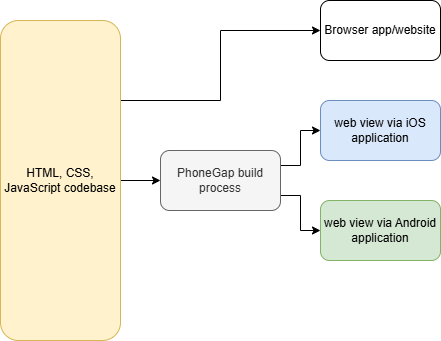
\includegraphics[width=0.5\linewidth]{litreview/images/phonegap.png}
    \caption{PhoneGap process}
    \label{fig:phonegap}
\end{figure}

The aforementioned PhoneGap, developed in 2008 by Nitobi Software, was the first major step in cross-platform development, and pioneered the `web app' approach described above. Nitobi Software was acquired by Adobe in 2011, and PhoneGap became part of Apache Cordova \cite{Apache-Cordova, Nitobi-Acquisition}. 



The first widely accepted approach for creating truly native cross-platform apps was React Native. Released in 2015, it extends the React JavaScript library and is written using the JSX extension for JavaScript \cite{React}. The React Native framework is still actively supported and maintained by Meta, along with the open-source community. React Native is able to render native UI from common source code by interpreting JSX code to create truly native code that is used to render UI components \cite{Danielsson2016}. 

This was closely followed by the release of Google's Flutter in 2017 \cite{Flutter-Release}. Flutter apps are built using the Google's Dart programming language, and instead of compiling to native code, apps ship with their own rendering engine \cite{Dart}. This approach has the benefit of being very performant, but the downside of not using truly native UI components. Flutter solves this problem by providing replicas of UI components for Android and iOS devices. 

\begin{figure}
    \centering
    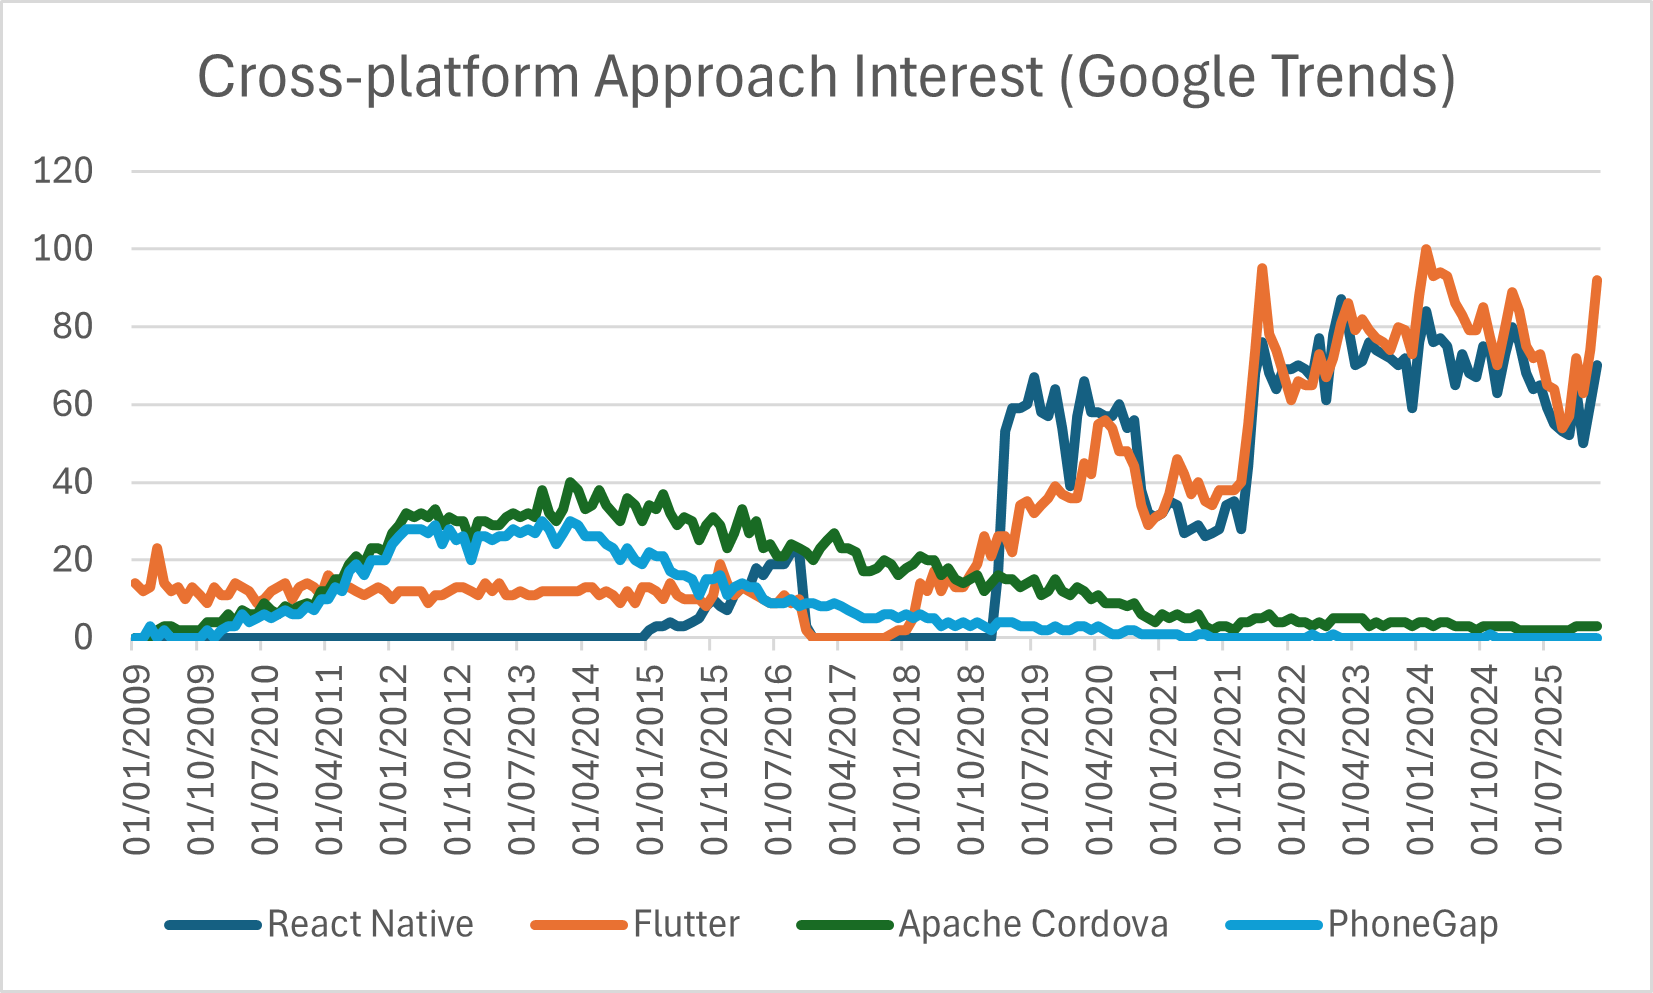
\includegraphics[width=0.5\linewidth]{litreview/images/cross_platform_trends.png}
    \caption{Search interest over time (data from \cite{google trends})}
    \label{fig:trends}
\end{figure}

\subsection{Cross-Platform Approach Comparison}

To deal with the problem of needing to develop applications for multiple different platforms, Heitkötter, Hanschke, and Majchrzak \cite{Heitkotter 2012} define three kinds of approaches: Web-based development, native development, and cross-platform approaches. A brief summary of each follows.

\begin{itemize}
    \item \textit{Web development}: Applications are developed as browser apps, which are then accessed via the device's browser application
    \item \textit{Native development}: Apps are created using the IDE associated with the target platform, e.g. Android Studio for Android, and XCode for iOS
    \item \textit{Cross-platform approaches}: A third-party framework is used to create a single codebase that is compiled or interpreted to native code
\end{itemize}

For this paper, we will be focusing on cross-platform approaches, with an emphasis on the process of writing one codebase that can be used to develop for different platforms.

It is important to define the criteria that will be used to evaluate cross-platform approaches, so that qualitative and quantitative observations and comparisons can be made. Jošt and Taneski \cite{Jost 2025} utilise data from developer surveys, community engagement and usage, and job market research, along with data from Google Trends to provide a numerical comparison of different approaches. This view of market and developer trends is useful as it can help developers choose a framework based on its current support and community, or its value in the job market.  Heitkötter, Hanschke, and Majchrzak based their evaluation on two sets of criteria one based on infrastructure, and one on development experience \cite{Heitkotter 2012}. The infrastructure criteria involve the features offered by the approach, the community and support available, and the potential quality of the apps that can be built with it. The development criteria focuses on the development environment, learning process, and development features such as graphical UI editors and simulators. Based on these examples, and independent research, the following criteria will be used to evaluate cross-platform approaches.

\begin{itemize}
    \item \textbf{Community and Support}: How `popular' is the app? Are there resources beyond the framework's documentation? Are there third party libraries and extensions available?
    \item \textbf{Framework Features}: The features the framework can produce in apps, e.g. native UI components, access to device-specific hardware such as the camera
    \item \textbf{Learning Curve}: The amount of new knowledge a developer must acquire to use this framework, and the extend to which that knowledge can be used in other contexts
    \item \textbf{Environment Features}: Features available during development, such as graphical UI editing, testing on simulators and real devices, third-party package management etc.
\end{itemize}

These criteria will be used to evaluate and compare the development frameworks themselves. Further criteria will be developed to evaluate the audio-specific results of different frameworks. For the `Community and Support' criteria, data will be gathered from \url{stackoverflow.com} regarding how many questions are being asked and answered online about each approach. 

\subsection{Audio Applications}

While there is a wealth of research done on the benefits, limitations, and options regarding cross-platform mobile development, there is a lack of information regarding audio development in this field. While audio processing is mentioned in some papers as an example of a complex real-time process that could require native code to reach performance requirements, there is no focus on the current tools and techniques for cross-platform audio development \cite{Patil 2025}. This is certainly an area in need of improvement, as mobile devices have become one of the most popular mode of listening to music, podcasts, audiobooks etc., along with becoming tools capable of complex audio recording and editing tasks.

% ----- IOS AUDIO DESCRIPTION ----- %

When developing audio applications for iOS, the immediately available solution is AVFAudio \cite{AVFAudio}. This is Apple's built in audio library for playing, recording, and processing audio. In a simple application, such as a music player app, a developer may only need to declare an \codeword{AVAudioPlayer} object and pass it an audio file to begin playback. These high level objects offer a comfortable level of abstraction from the underlying audio graph, while still providing adequate control for simple applications. If the application calls for more advanced control, such as live processing or synthesis, AVFAudio provides access to the audio graph via the \codeword{AVAudioEngine}. The audio graph is a sequence of connected 'nodes' that take audio input, process it, and render it to an output. The developer can create nodes in this graph that synthesise and process audio. Real-time processing and effects need to be done as efficiently as possible, so they are written as C++ classes, with an Objective-C adapter class to allow the app's Swift code to communicate with them \cite{AVFAudioEffects}. High level third-party libraries are also available for developers. The free and open-source AudioKit project provides the same recording, playback, and processing capabilities as AVFAudio, but with many more effects and functionalities built in \cite{AudioKit}. AudioKit works by wrapping AVFAudio objects in a layer of abstraction, making it easier to build a complex audio graph, providing many useful effect and processing nodes so that the user does not need to create them from scratch. AudioKit also offers a graphical extension for that allows the user to create their processing chain with minimal code \cite{AudioKitFlow}. AudioKit objects do provide access to the underlying AVAudioNodes that they are build with.

\begin{figure}
    \centering
    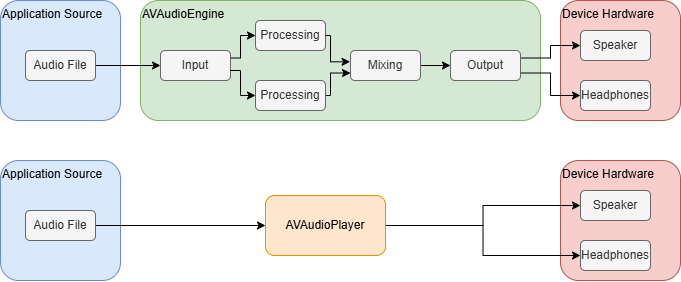
\includegraphics[width=0.5\linewidth]{litreview/images/AVFAudio.png}
    \caption{High level (top) and low level (bottom) audio control with AVFAudio}
    \label{fig:AVFAudio}
\end{figure}

% ----- ANDROID AUDIO DESCRIPTION ----- %

Android audio development is similar to that of iOS, in that a build in library (android.media) is immediately available to the developer \cite{android.media}. The user may only need to declare \codeword{MediaPlayer} and \codeword{MediaRecorder} objects for playback and recording, respectively. The \codeword{android.media} library does provide some basic audio effects, such as equalization and reverb. In the documentation for these effects it is recommended that developers use the premade effect classes rather than implementing their own using the \codeword{AudioEffect} class. Since Android apps are written in Java or Kotlin, and the underlying code that accesses hardware is written in C++, a JNI is necessary to access the device's hardware abstraction layer (HAL), as seen in fig. \ref{fig:android audio}\cite{android audio}. These layers of abstraction create latency and make the default audio api unsuitable for real-time processing \cite{Balsini 2019}. 

% ----- CROSS PLATFORM AUDIO DESCRIPTION ----- %

When using a cross platform approach, it is obviously much more difficult to have low-level control over audio. The differences in the hardware and the way audio is processed on different platforms is great enough that a high level of abstraction is required to create code that will work on multiple platforms. Luckily, there are many solutions available for platforms like React Native and Flutter, due to their large and active communities. From a review of some popular libraries, it seems that most offer a similar functionality to the native solutions, with recording, playback, and basic processing available at a high level \cite{rnaudioapi, flutteraudio}. Research regarding the extend of low-level control and real-time processing that is possible will be conducted. 


\begin{figure}
    \centering
    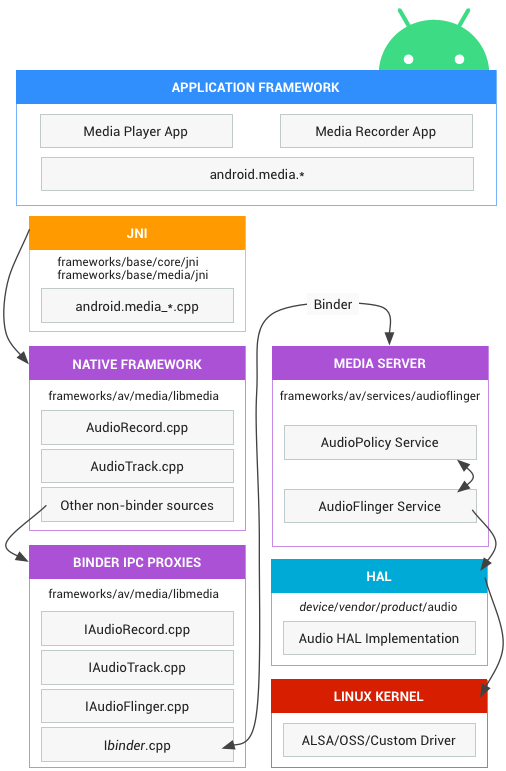
\includegraphics[width=0.5\linewidth]{litreview/images/ape_fwk_audio.png}
    \caption{Android audio architecture (via \cite{android audio})}
    \label{fig:android audio}
\end{figure}

